\section{Empirical applications}\label{sec:empirical}

We compare short-memory and plug-in critical values on three contiguous series (\cref{fig:empirical,tab:empirical}).
The examples span local Whittle estimates of $H$ from \pthree{emp-aus-hlw} to \pthree{emp-nile-hlw}.
\begin{enumerate}
\item \emph{New South Wales electricity demand.} We aggregate half-hourly load from the Monash archive \citep{God21,MonashNSW}
to daily energy $D_t$ and test whether mean year-over-year growth $100\log(D_t/D_{t-365})$ is zero.
The $1095$ observations from March 2012 to February 2015 average \pthree{emp-aus-xbar}\,\%.
\item \emph{London air quality.} At Greenwich--Westhorne Avenue (GR9), we take the logarithm of each daily mean
$\mathrm{PM}_{2.5}$ concentration, in $\mu\mathrm{g}/\mathrm{m}^3$. From 1 January 2017 to 30 March 2018,
all 454 days have observations. The hourly archive \citep{MonashGR9} has 76 missing readings across 32 of those days;
each daily mean uses the available hours. We compare the geometric mean with two illustrative reference
concentrations, 10 and 15. The sample geometric mean is \pthree{emp-lon-geom}, and the arithmetic mean is
\pthree{emp-lon-arith}\,$\mu\mathrm{g}/\mathrm{m}^3$.
\item \emph{Nile annual minima.} The Roda Gauge series comprises 663 annual minimum water levels from AD 622 to 1284
\citep{Tou25,Hur51,Ber94}. We use 1100\,cm as a reference and obtain a sample mean of \pthree{emp-nile-xbar}\,cm.
\end{enumerate}

In \cref{fig:empirical}, coloured end marks identify plug-in intervals that change the decision relative to the grey interval.
For the plug-in tests, the archive interpolates the critical value at $\hat H_{\mathrm{LW}}$. It encloses the
limiting tail probability with $H$ fixed at that estimate rounded to four decimal places. These bounds quantify
numerical error. The sampling variability of $\hat H$ affects the rejection rates of feasible tests
(\cref{sec:competitors}). The last column of \cref{tab:empirical} gives the rejection rate of the short-memory cutoff
under a fitted Gaussian ARFIMA$(0,\hat d_{\mathrm{LW}},0)$ model. Daggers identify changed decisions at $5\,\%$;
the interval ratio is plug-in width divided by short-memory width. MAC and subsampling use their own reference laws.

\begin{figure}[tbp]\centering
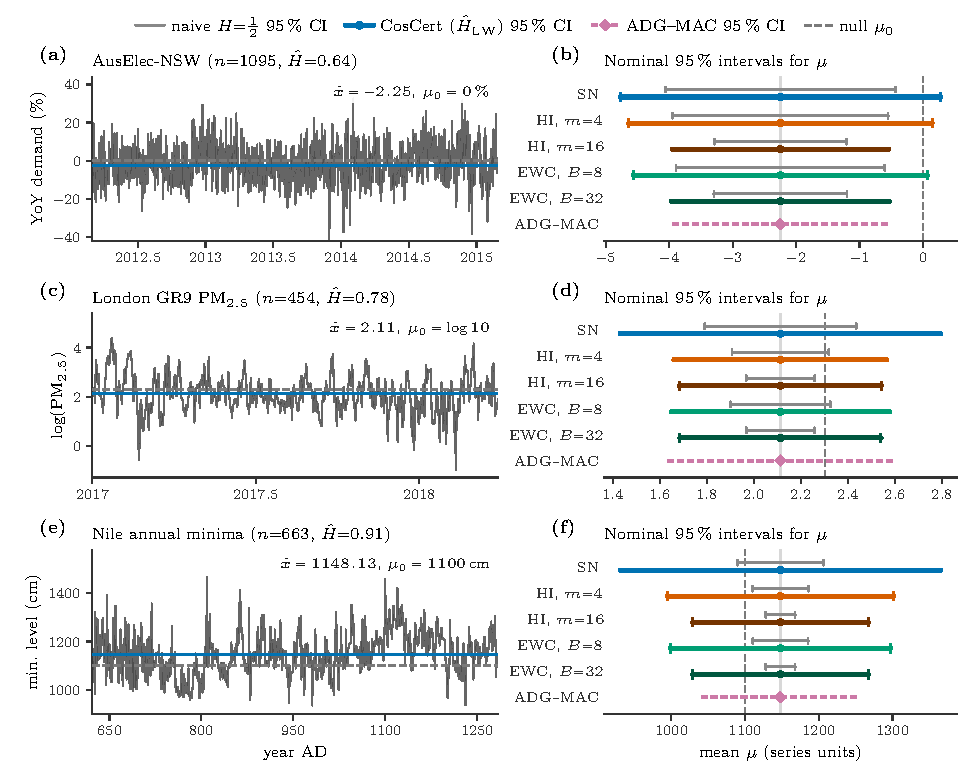
\includegraphics[width=\textwidth]{fig7_empirical.pdf}
\caption{Observed series and nominal 95\% intervals for mean electricity growth, log particulate concentration and Nile minima.}\label{fig:empirical}
\end{figure}

\begin{table}[tbp]\centering\small
\caption{Short-memory and plug-in tests of three series means. Daggers mark decisions that change at 5\%.}\label{tab:empirical}
\footnotesize\setlength{\tabcolsep}{2.2pt}\begin{tabular}{@{}llrrrrrrr@{}}\toprule
series & test & stat & \multicolumn{2}{c}{$5\,\%$ cutoff} & \multicolumn{2}{c}{$p$-value} & CI & naive\\
\cmidrule(lr){4-5}\cmidrule(lr){6-7}
($\hat H_{\mathrm{LW}}/\hat H_{\mathrm{ELW}}$, $n$, $\mu_0$) & & & naive & \CosCert{} & naive & \CosCert{} & ratio & size (\%)\\\midrule
AusElec-NSW & SN$^\dagger$ & 70.19 & 45.53 & 88.83 & 0.022 & 0.071 & 1.40$\times$ & 12.1\\
$\hat H{=}0.641/0.645$ & HI, $m{=}4$$^\dagger$ & $-3.05$ & 2.31 & 3.25 & 0.016 & 0.062 & 1.41$\times$ & 14.0\\
$n{=}1095$, $\mu_0{=}0\,\%$ & HI, $m{=}16$ & $-4.40$ & 2.04 & 3.34 & $<0.001$ & 0.012 & 1.64$\times$ & 22.3\\
 & EWC, $B{=}8$$^\dagger$ & $-3.15$ & 2.31 & 3.25 & 0.014 & 0.056 & 1.41$\times$ & 14.0\\
 & EWC, $B{=}32$ & $-4.37$ & 2.04 & 3.34 & $<0.001$ & 0.012 & 1.64$\times$ & 22.3\\
 & ADG--MAC / Sub.\ SN & $-2.58$ / -- & \multicolumn{2}{c}{1.96 / --} & \multicolumn{2}{c}{0.010 / 0.135} & -- & --\\
\midrule
London GR9 & SN & 15.73 & 45.53 & 204.04 & 0.192 & 0.454 & 2.12$\times$ & 24.6\\
$\hat H{=}0.784/0.791$ & HI, $m{=}4$ & $-2.12$ & 2.31 & 5.07 & 0.067 & 0.361 & 2.20$\times$ & 32.3\\
$n{=}454$, $\mu_0{=}\log 10$ & HI, $m{=}16$$^\dagger$ & $-2.65$ & 2.04 & 6.00 & 0.012 & 0.373 & 2.95$\times$ & 49.2\\
 & EWC, $B{=}8$ & $-2.06$ & 2.31 & 5.05 & 0.074 & 0.373 & 2.19$\times$ & 32.1\\
 & EWC, $B{=}32$$^\dagger$ & $-2.65$ & 2.04 & 5.99 & 0.012 & 0.371 & 2.94$\times$ & 49.1\\
 & ADG--MAC / Sub.\ SN & $-0.77$ / -- & \multicolumn{2}{c}{1.96 / --} & \multicolumn{2}{c}{0.440 / 0.276} & -- & --\\
\midrule
Nile minima & SN & 30.98 & 45.53 & 632.75 & 0.089 & 0.522 & 3.73$\times$ & 44.9\\
$\hat H{=}0.909/0.908$ & HI, $m{=}4$$^\dagger$ & 2.91 & 2.31 & 9.26 & 0.020 & 0.482 & 4.02$\times$ & 57.5\\
$n{=}663$, $\mu_0{=}1100\,\mathrm{cm}$ & HI, $m{=}16$$^\dagger$ & 4.92 & 2.04 & 12.18 & $<0.001$ & 0.409 & 5.98$\times$ & 73.0\\
 & EWC, $B{=}8$$^\dagger$ & 2.96 & 2.31 & 9.19 & 0.018 & 0.471 & 3.99$\times$ & 57.2\\
 & EWC, $B{=}32$$^\dagger$ & 4.92 & 2.04 & 12.15 & $<0.001$ & 0.408 & 5.97$\times$ & 73.0\\
 & ADG--MAC / Sub.\ SN & 0.88 / -- & \multicolumn{2}{c}{1.96 / --} & \multicolumn{2}{c}{0.381 / 0.272} & -- & --\\
\midrule
London GR9 & SN$^\dagger$ & 155.15 & 45.53 & 204.04 & 0.003 & 0.073 & 2.12$\times$ & 24.6\\
$\hat H{=}0.784/0.791$ & HI, $m{=}4$ & $-6.66$ & 2.31 & 5.07 & $<0.001$ & 0.016 & 2.20$\times$ & 32.3\\
$n{=}454$, $\mu_0{=}\log 15$ & EWC, $B{=}8$ & $-6.46$ & 2.31 & 5.05 & $<0.001$ & 0.019 & 2.19$\times$ & 32.1\\
 & ADG--MAC / Sub.\ SN & $-2.42$ / -- & \multicolumn{2}{c}{1.96 / --} & \multicolumn{2}{c}{0.015 / 0.005} & -- & --\\
\bottomrule\end{tabular}
%
\end{table}

In New South Wales all five tests reject zero mean growth with the short-memory cutoffs. With plug-in calibration,
three change decision: SN ($p=\pthree{emp-aus-SN-pcc}$), HI with $m=4$ ($p=\pthree{emp-aus-HI4-pcc}$)
and EWC with $B=8$ ($p=\pthree{emp-aus-EWC8-pcc}$). HI with $m=16$ and EWC with $B=32$ still reject.
The choice of smoothing therefore matters even when the memory estimate is held fixed.

For London, HI with $m=16$ changes from $p=\pthree{emp-lon-HI16-pnv}$ to $p=\pthree{emp-lon-HI16-pcc}$
at the reference concentration of 10. At the reference of 15, SN gives $p=\pthree{emp-lon15-SN-pcc}$,
while HI with $m=4$ and EWC with $B=8$ give $p=\pthree{emp-lon15-HI4-pcc}$ and
$p=\pthree{emp-lon15-EWC8-pcc}$. These comparisons concern the mean of log concentration over the observed period.

For the Nile, all four fixed-smoothing tests change from rejection to non-rejection. The widest relative change
occurs for HI with $m=16$: its interval expands by a factor of \pthree{emp-nile-HI16-ratio}, and its plug-in
$p$-value is \pthree{emp-nile-HI16-pcc}. LW and demeaned ELW give the same decisions in all three series.

\FloatBarrier
